\documentclass[a4paper,12pt]{article}
\usepackage[utf8]{inputenc}
\usepackage{fontenc}
\usepackage{graphicx}
\usepackage{scrextend}
\usepackage{tikz}
\usepackage{pgfplotstable}%color table
\usepackage{xspace}
\usepackage{url}


\def\cnb{CNB\xspace}

\newcommand{\ffigure}[1]{Figure \ref{#1}}
\newcommand{\ttable}[1]{Table \ref{#1}}
\newcommand{\ffigures}{Figures}
\newcommand{\ttables}{Tables}
\def\scipionbox{\textit{ScipionBox}\xspace}
\def\mnas{\textit{microscope-NAS}\xspace}
\def\onas{\textit{Output-NAS}\xspace}
\def\hserver{\textit{HTML-Server}\xspace}
\def\scipion{\textit{Scipion}\xspace}
\def\emadmin{\textit{EMAdmin}\xspace}
\def\python{\textit{Python}\xspace}

\def\epu{\textit{EPU}\xspace}
\def\scilifelab{SciLifeLab\xspace}
\def\cnbcsic{CNB-CSIC\xspace}
\def\cnb{CNB\xspace}

\date{06/09/18}
% response_macros.tex
\newcommand{\initresponses}{\newcounter{pointcounter}}

\newenvironment{reviewer}{\setcounter{pointcounter}{1}}{}

\newcommand{\point}[1]{\medskip \noindent
               \textsl{{\fontseries{b}\selectfont Q\thepointcounter}.
                 \stepcounter{pointcounter} #1}}
\newcommand{\reply}{\medskip \noindent \textbf{Answer}.\ }

\initresponses


\begin{document}


\begin{reviewer}
\section*{Reviewer 1}
\point{The graphical abstract is likely too detailed 
and would not show well when reduced to the image size that the final version has.}

\reply  Both reviewers complain that the graphical abstract need to be redesigned. The first reviewer complains that is ``...too detailed...'' while the second one claims that ``...is oversimplified...''. Since the graphical abstract is not compulsory  and both reviewers dislike it for completely opposite and irreconcilable reasons we have decided to drop it.


\point{The manuscript would benefit from a figure that outlines the layout of a typical Scipion system, showing computers, data connections, data flows in workflow scenarios, and how streaming is now implemented. At least for one of the three examples described, a figure would be helpful and make the manuscript more appealing to readers. }

\reply The following figure has been included in the manuscript. 

\begin{figure}
  \centering
      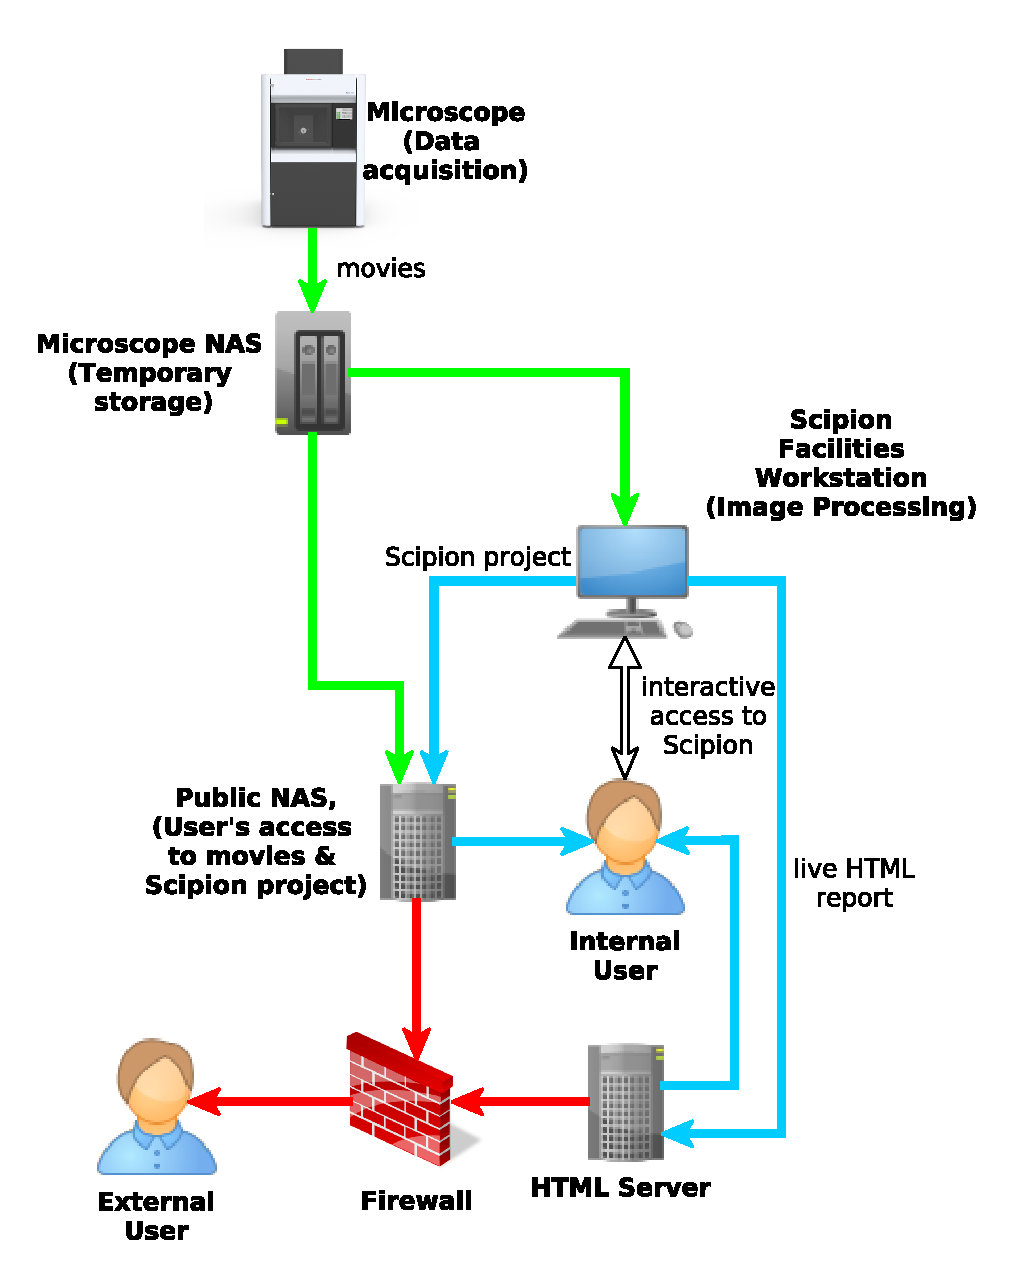
\includegraphics[width=0.75\textwidth]{images/diagram.pdf}
  \caption{Graphical representation of the data flow through the CNB facility. Green, blue and red lines represent the microscope private network, the \cnb local area network and the public network respectively.}
  \label{fig:cnbpipeline}

\end{figure}
\clearpage

%\point{The English language at a few locations would benefit from further proof reading, but these are minor problems. }

%\reply tut-tuc-tuc 

% The English language at a few locations would benefit from further proof reading, but these are minor problems. 
% 
% E.g.:
% There are two different abstracts provided. One in the PDF for reviewing, and a second, shorter Abstract at the beginning of the manuscript text. 
% For the first Abstract: "… how the execution of the algorithms is going on" would be better phrased "… how the execution of the algorithms is progressing".
% For the second Abstract: "and it is being considered in many more." is a claim, not a provable fact. It should not be stated here. Even though, this statement might be true, the same would apply to all other software systems, which are likely being considered somewhere. 
% 
% Page 4: "Stream processing, i.e. computing" should be "Stream processing, i.e., computing" (comma missing). 
% 
% Page 6: "we described the pipeline offered…" should be "we describe the pipeline offered…"
% 
% Page 9: "by any user which…" should be "by any user, who…"
% Same page: Explain what EPU is.
% 
% Page 10: "Weak ciphers (as arcfour) has been activated…" Should this be "Weak ciphers have been activated…"?   Please explain, what ciphers are.
% 
% Page 11 and in a few locations thereafter: "You are welcomed to download…" is awkwardly phrased. It should be "You are welcome to download…", but even then, it should be better stated as "The software can be freely downloaded and customized to meet the specific requirements of client organizations."
% 
% Page 13:  "Thermofisher Titan Krios" should probably be "Thermo Fischer Scientific Titan Krios" or "Thermo Scientific Titan Krios". 
% 
% Page 16: The sentence "They can potentially play with the pipeline in ways that are not possible when having a programmer writing the code for them." Is not understandable on first reading. Do you mean "This allows users to adjust the pipeline, which would not be possible with hard-coded workflows."
% 
% Page 17: "her home institution" should be "his/her home institution".

\point{Minor corrections in pages: Abstract, 4, 6, 9, 10, 11, 13, 16, 17}

\reply All grammar, spelling typos, rephrasing and other minor corrections suggested by the reviewer have been followed except one. Below we comment on the non followed suggestions (page 9 and 10) and the modifications introduced in page 16 since involve the rewriting of a paragraph. 

Q \the\numexpr\value{pointcounter}-1\relax.1: Page 9: ``...Explain what EPU is...''. EPU has already been introduced by the following two paragraphs.

\begin{quote}
 Many software packages have been developed to support automated data collection, such as 
 .., EPU (Thermo Fisher Scientific, 2018), ..., etc.
\end{quote}

\begin{quote}
...we comment on an additional software (called  \emadmin) that connects \scipion with the microscope acquisition software (\epu) and records the facility activity.
\end{quote}

Q \the\numexpr\value{pointcounter}-1\relax.1: Page 10: ``Please explain, what ciphers are''. Following reviewer 2 recommendations this section has been simplified and the sentence containing the word ``ciphers'' has been deleted. 

Q \the\numexpr\value{pointcounter}-1\relax.2: Page 16: ``The sentence -They can potentially play with the pipeline in ways that are not possible when having a programmer writing the code for them.- Is not understandable on first reading.''. We have rewritten the paragraph as:


\begin{quote}
 Workflows implement pipelines and describe them as a set of interconnected steps. In a workflow approach, users (including microscope staff) can reasonably be expected to modify the paths and incorporate new steps using a GUI. Alternate solutions as scripts do not clearly separate each step definition from the connections between the different steps and, for no programmers, are scary and difficult to modify. 
\end{quote}

\end{reviewer}

\begin{reviewer}
\section*{Reviewer 2}

\point{The authors claim that the strength of their software is in its ability to process data while being collected; a point that is not well-addresses by other software. At the same time, they acknowledge that UCSFImage4, Focus, and Relion are software packages similar to Scipion capable of processing data in a high-throughput manner while new data is being acquired at the microscope. A clear differentiation between Scipion and these software packages was lacking in this manuscript. What advantages Scipion provide over the above mentioned software packages?}


\reply %Since there is already a published manuscript describing \scipion, in the present manuscript  we decided to focus on \scipion features that have been specifically developed for working at EM facilities (e.g. streaming). The main reasons why \scipion is better suited than other packages for EM work is rooted in \scipion main design, complimented with the new facilities related features. Nevertheless, 
The reviewer is right in pointing out than a ``A clear differentiation between \scipion and these software packages was lacking in this manuscript''. Therefore, we have decided to add the following subsection to the manuscript

\begin{quote}

\textbf{\scipion Design and Architecture}

We would like to finish this section commenting on some of \scipion  design decisions that differentiate \scipion from other image processing frameworks. \scipion
is fully oriented to integrate existing
EM software and therefore the versatility and number of possible steps
combination is huge. Additionally, \scipion takes care of keeping a 
rigorous traceability and reproducibility as well as to provide an API (application programming interface) to allow the integration  with already existing LIMS systems. At the software architectural level,  the greatest difference 
between \scipion and the other EM image processing packages mentioned in the introduction 
is that  \scipion pays special attention to define abstraction layers to simplify maintenance
and extensibility and follows a strict workflow approach. A few examples will illustrate the main advantages of this approach.

To create a new protocol in \scipion, a single \python file needs to be created. From this file, the system will discover the new protocol and will automatically build
a form and store the protocol related information in a database.
\scipion protocol developers must certainly know \scipion conventions
but they do not need to modify or even understand the existing code.
In  \scipion next version, the abstraction will be increased
since protocols will be implemented as plug-ins,
that is, independent small \python files  that add functionality to the main
\scipion application. The plug-in approach allows parallel development. That is,  
since protocols are implemented independently from the main application
they can be developed and released in parallel by different teams. In this way, support for a new version of \textit{Relion} does not require a new \scipion release but
a release of the independent \textit{Relion} plug-in

\scipion follows a pure workflow approach and therefore, implements pipelines and describes them as a set of interconnected steps (or protocols). In a workflow approach, users (including microscope staff) can reasonably be expected to modify the paths and incorporate new steps using a GUI (graphic user interface). On the contrary, software packages that do not make this separation produce workflows that, in general, are more challenging to create or modify for non programmers. 

Another advantage of a clear separation between steps and relationships 
is the improvement of load balance, reproducibility and  provenance (process of tracing and recording the origins of data and its movement between protocols). The first step in a \scipion workflow execution
is to store in a database each of the protocols to be executed as well as how 
outputs of one protocol are attached to the inputs of another protocol. Then, a workflow engine analyzes the stored data and, using as constraint the number of CPUs assigned by the user to the workflow, optimizes the execution, that is, tries to execute as many protocols in parallel as possible. Obviously, the data stored in the database  have enough information to execute each step and therefore guarantee reproducibility and provenance. Additionally, \scipion currently exports a JSON (JavaScript Object Notation) file describing the complete preprocessing workflow used, so that it can be fully reproduced and visualized elsewhere.

\end{quote}


%In Appion, however, the developer must develop the script, the cor-
%responding form, and an extra table in the database; 
%Appion developers might thus need to know the underlying framework in more
%detail.

%It is difficult to predict how EM software will evolve in the
%future. Our view is that software developers will continue to add
%algorithms to the different EM packages, but that the burden of
%many operations will be shifted from packages to frameworks.
%Bookkeeping will require special attention to provide real tracking
%and reproducibility. Workflows will have a key role when explor-
%ing processing alternatives. Most algorithms will need to use dis-
%tributed computing through clusters or the Cloud. Scipion is our
%first step in implementing an integrative framework to address
%important problems in the field simply and effectively

\point{The authors mentioned that Scipion has been installed and in production mode in seven facilities. Is there a way to know how Scipion is being used and to get statistical data on its usage?}

\reply The following paragraphs have been added in the manuscript.

\begin{quote}

In the context of free and open source projects it is difficult to create usage statistics that are accurate. But certainly, if we want \scipion to succeed, we need to 
know how frequent the different protocols are used. This is the reason why we have recently developed our \textit{Scipion Usage Data Collector} that monitors -if activated by the user- the usage of the different protocols and send -via HTTP protocol- the information to the developer's team. This information is anonymous and cannot be used to identify the original computer in which \scipion has been executed. 

Using the HTTP header it is possible to guess the country in which \scipion has been installed. With these information we have created the usage map and table available at URL \url{http://scipion.i2pc.es/report_protocols/scipionUsage/} and  \url{http://scipion.i2pc.es/report_protocols/protocolTable/}. The data corresponds on ``global'' \scipion usage rather than ``facility'' usage but there 
is a one to one relationship between the  countries with highest number of \scipion projects and the countries with \scipion based EM facilities. The only exception to the rule is Canada where two of the original \scipion developers are setting up a new facility (McGill University).

Note that, in a effort to report real use and skip test projects, the number of projects in the map refers to the number of non empty \scipion projects updated more than once. That is, 
\scipion projects that have been opened in at least two different days. Another constraint is that developers' computers are filtered out.
\end{quote}


\point{Section 4 on Scipion setup at different facilities was confusing and unnecessarily lengthy. It wasn't clear to me if the "Additional software developments" made in 4.1.2 and 4.2.2 were general to Scipion or only made as a case-by-case scenario?}

\reply Section 4 has been extensively rewritten to take into account the reviewers' suggestions. In summary, we have included a new image, delete several paragraphs, modify others and move those paragraphs related with future work to a different section.

Please confer the file ``Revised Manuscript(marked)'' attached to this review in which 
all significant differences between the original manuscript and the revised one are marked up.

Q \the\numexpr\value{pointcounter}-1\relax.1: ``It wasn't clear to me if the Additional software developments made in 4.1.2 and 4.2.2 were general to Scipion or only made as a case-by-case scenario?''. The following paragraph have been modified.

\begin{quote}
 This section in divided in two parts. In the first one we discuss the network setup that allows us to move the data from the microscope to the user laboratory. Then,  we comment on an additional software called  \emadmin. \emadmin has been specifically designed for the \cnb facility, it connects \scipion with the microscope acquisition software (\epu) and records the facility activity.
\end{quote}


\point{The graphical abstract is oversimplified and does not convey any of the useful information presented in the manuscript. The background is distracting, the cartoons are redundant with the labels, and the image describing the reporting feature is not legible and improperly sized (laterally stretched).}

\reply See answer to reviewer 1 question 1. 

\point{Finally, the manuscript could benefit greatly from more visual summaries and schematics to guide the readers especially the non-experts that the authors refer to as part of their target consumer base.}

\reply We think the reviewer refer here to section 4. As commented previously this section has been extensively rewritten to take into account the reviewers' suggestions and it includes a new figure.

\end{reviewer}
\end{document}
